% (The MIT License)
%
% Copyright (c) 2023-2024 Yegor Bugayenko
%
% Permission is hereby granted, free of charge, to any person obtaining a copy
% of this software and associated documentation files (the 'Software'), to deal
% in the Software without restriction, including without limitation the rights
% to use, copy, modify, merge, publish, distribute, sublicense, and/or sell
% copies of the Software, and to permit persons to whom the Software is
% furnished to do so, subject to the following conditions:
%
% The above copyright notice and this permission notice shall be included in all
% copies or substantial portions of the Software.
%
% THE SOFTWARE IS PROVIDED 'AS IS', WITHOUT WARRANTY OF ANY KIND, EXPRESS OR
% IMPLIED, INCLUDING BUT NOT LIMITED TO THE WARRANTIES OF MERCHANTABILITY,
% FITNESS FOR A PARTICULAR PURPOSE AND NONINFRINGEMENT. IN NO EVENT SHALL THE
% AUTHORS OR COPYRIGHT HOLDERS BE LIABLE FOR ANY CLAIM, DAMAGES OR OTHER
% LIABILITY, WHETHER IN AN ACTION OF CONTRACT, TORT OR OTHERWISE, ARISING FROM,
% OUT OF OR IN CONNECTION WITH THE SOFTWARE OR THE USE OR OTHER DEALINGS IN THE
% SOFTWARE.

\documentclass{article}
\usepackage{../sqm}
\newcommand*\thetitle{Builds}
\begin{document}

\plush{\sqmTitlePage{21}{}}

\qte
  [Martin Fowler]
  {../06-coupling/martin-fowler.jpg}
  {For most projects, the XP guideline of a \ul{ten minute} build is perfectly within reason. Most of our modern projects achieve this. It's worth putting in concentrated effort to make it happen, because every minute chiseled off the build time is a minute \ul{saved} for each developer every time they commit.}
  {fowler2006}

\qte
  [Kai Huang]
  {kai-huang.jpg}
  {Our results show there are good reasons for the rise of CI. Compared to projects that do not use CI, projects that use CI: \ul{release} twice as often, \ul{accept pull requests} faster (1.6x), and have developers who are \ul{less worried} about breaking the build.}
  {hilton2016usage}
\pitch{\begin{multicols}{2}
  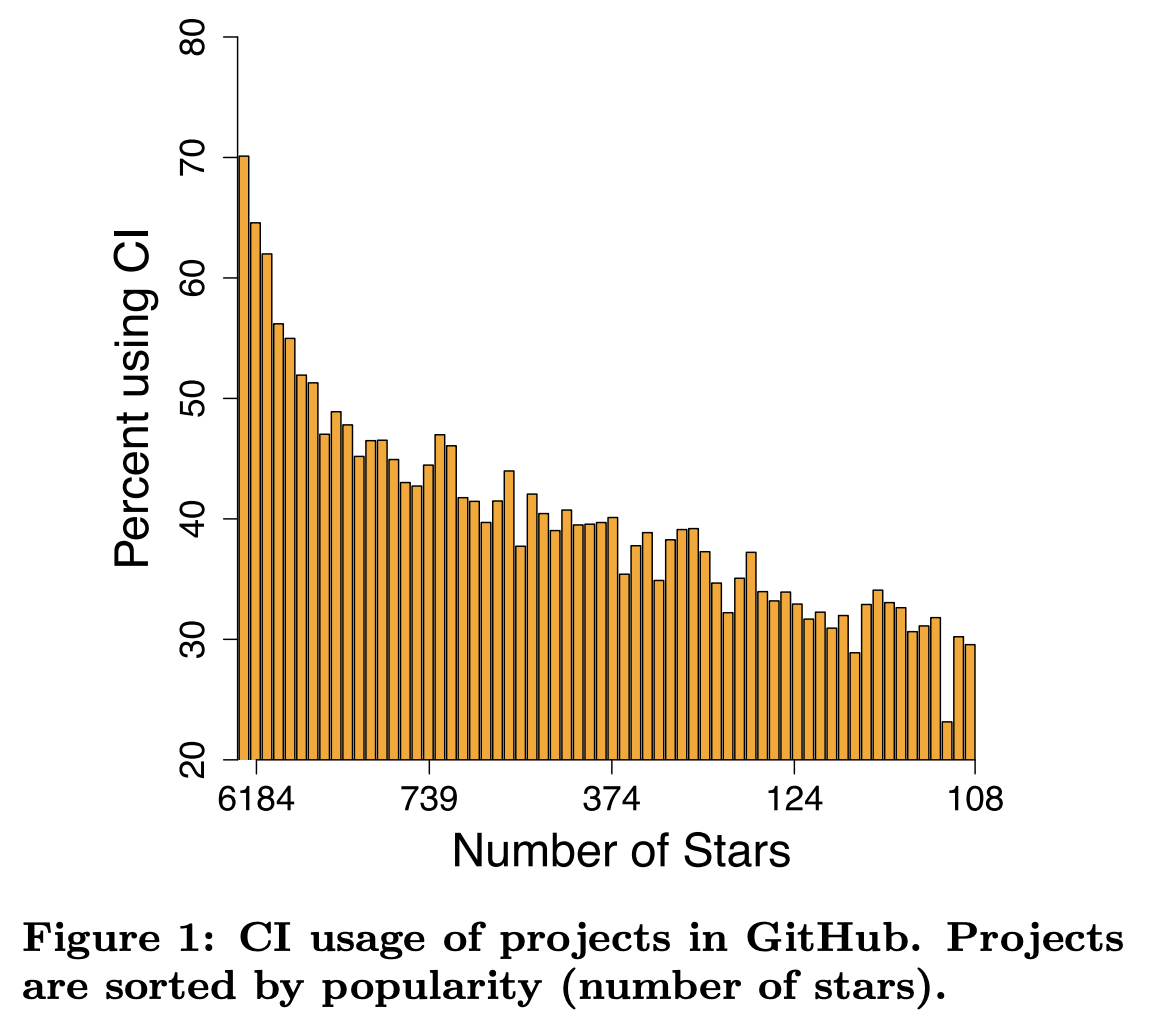
\includegraphics[width=.9\linewidth]{by-stars.png}
  \par\columnbreak\par
  ``In the most popular (starred) group, 70\% of projects use CI. As the projects become less popular, the percentage of projects using CI declines to 23\%. Observation: Popular projects are more likely to use CI.''
  \source{hilton2016usage}
  \end{multicols}}
\pitch{\begin{multicols}{2}
  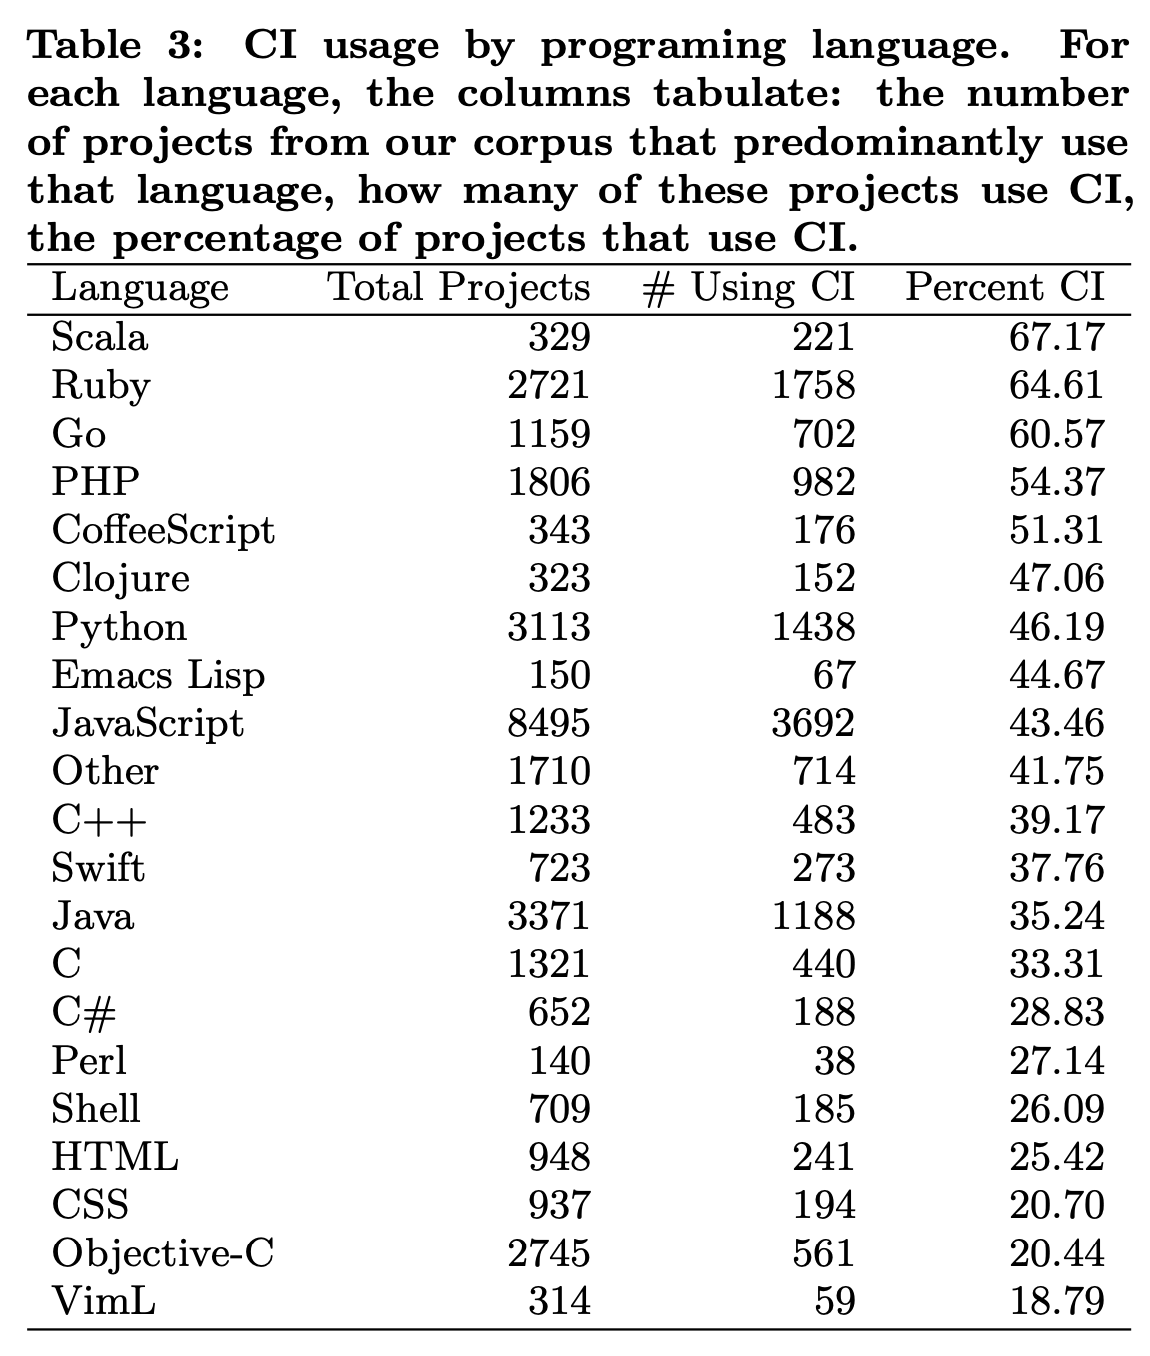
\includegraphics[width=.8\linewidth]{by-language.png}
  \par\columnbreak\par
  ``Languages that have the highest CI usage are also dynamically-typed (e.g., Python and JavaScript). One possible explanation may be that in the absence of a static type system which can catch errors early on, these languages use CI to provide extra safety.''
  \source{hilton2016usage}
  \end{multicols}}
\pitch{\begin{multicols}{2}
  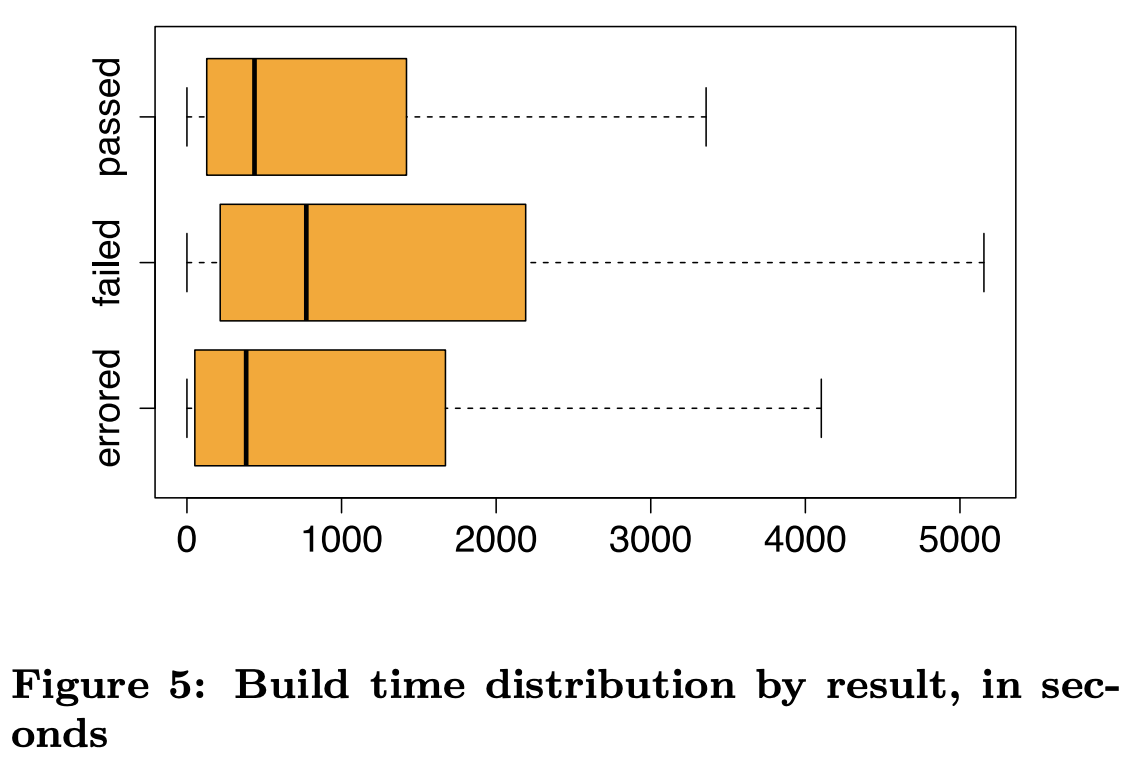
\includegraphics[width=.9\linewidth]{duration.png}
  \par\columnbreak\par
  ``The average build time is just under 500 seconds. Errored builds are those that occur before the build begins (e.g., when a dependency cannot be downloaded), and failed builds are those that the build is not completed successfully.''
  \source{hilton2016usage}
  \end{multicols}}

\qte
  [Michael Hilton]
  {michael-hilton.jpg}
  {Developers use CI to guarantee \ul{quality}, consistency, and viability across different environments. However, adding and maintaining automated tests causes these benefits to come at the expense of \ul{increased time} and \ul{effort}.}
  {hilton2017trade}
\pitch{\begin{multicols}{2}
  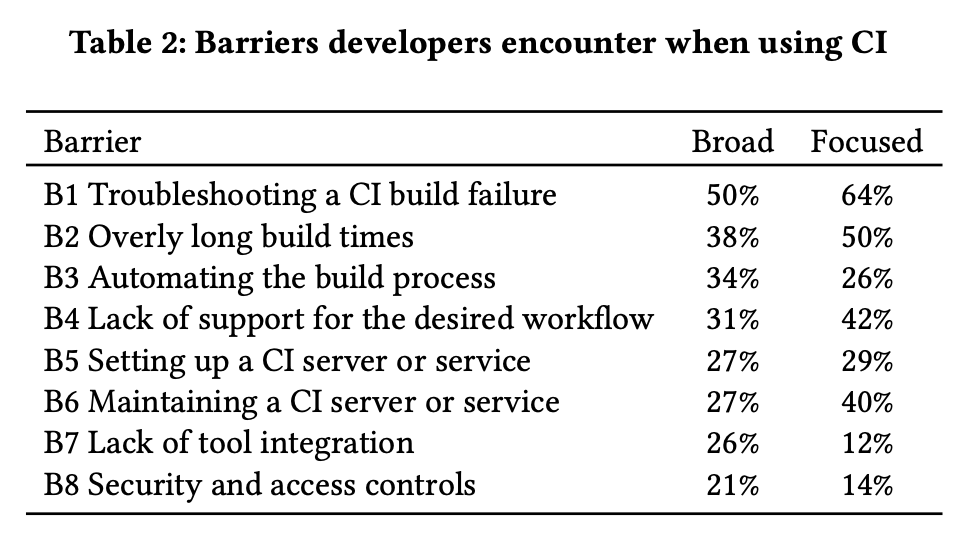
\includegraphics[width=.9\linewidth]{barriers.png}
  \par\columnbreak\par
  ``When a CI build fails, some participants begin the process of identifying why the build failed. \ul{Sometimes}, this can be fairly straightforward...''
  \source{hilton2017trade}
  \end{multicols}}
\pitch{\begin{multicols}{2}
  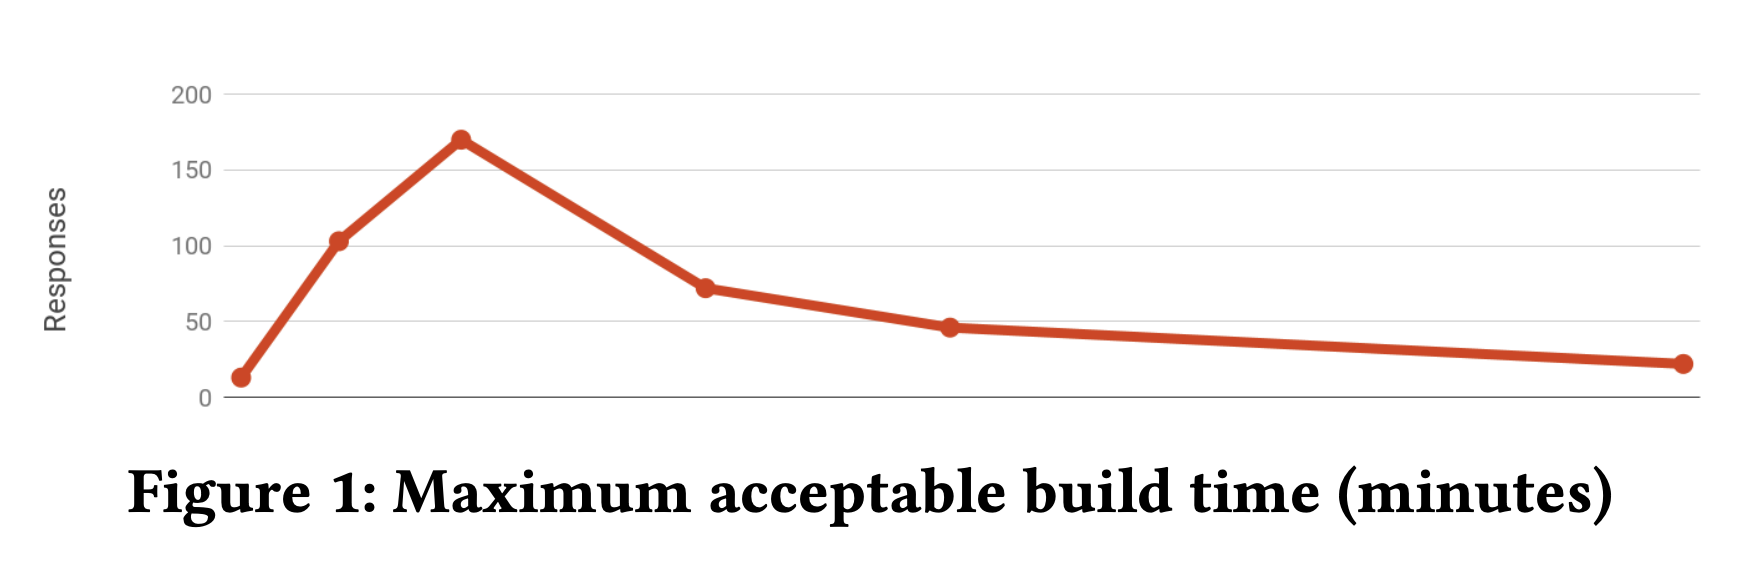
\includegraphics[width=.9\linewidth]{ten-minutes.png}
  \par\columnbreak\par
  ``\citep{fowler2006} suggests most projects should try to follow the XP guideline of a 10-minute build. When we asked our 523 participants what is the \ul{maximum acceptable time} for a CI build to take, the \ul{most common answer} was also 10 minutes.''
  \source{hilton2017trade}
  \end{multicols}}
\pitch{\begin{multicols}{2}
  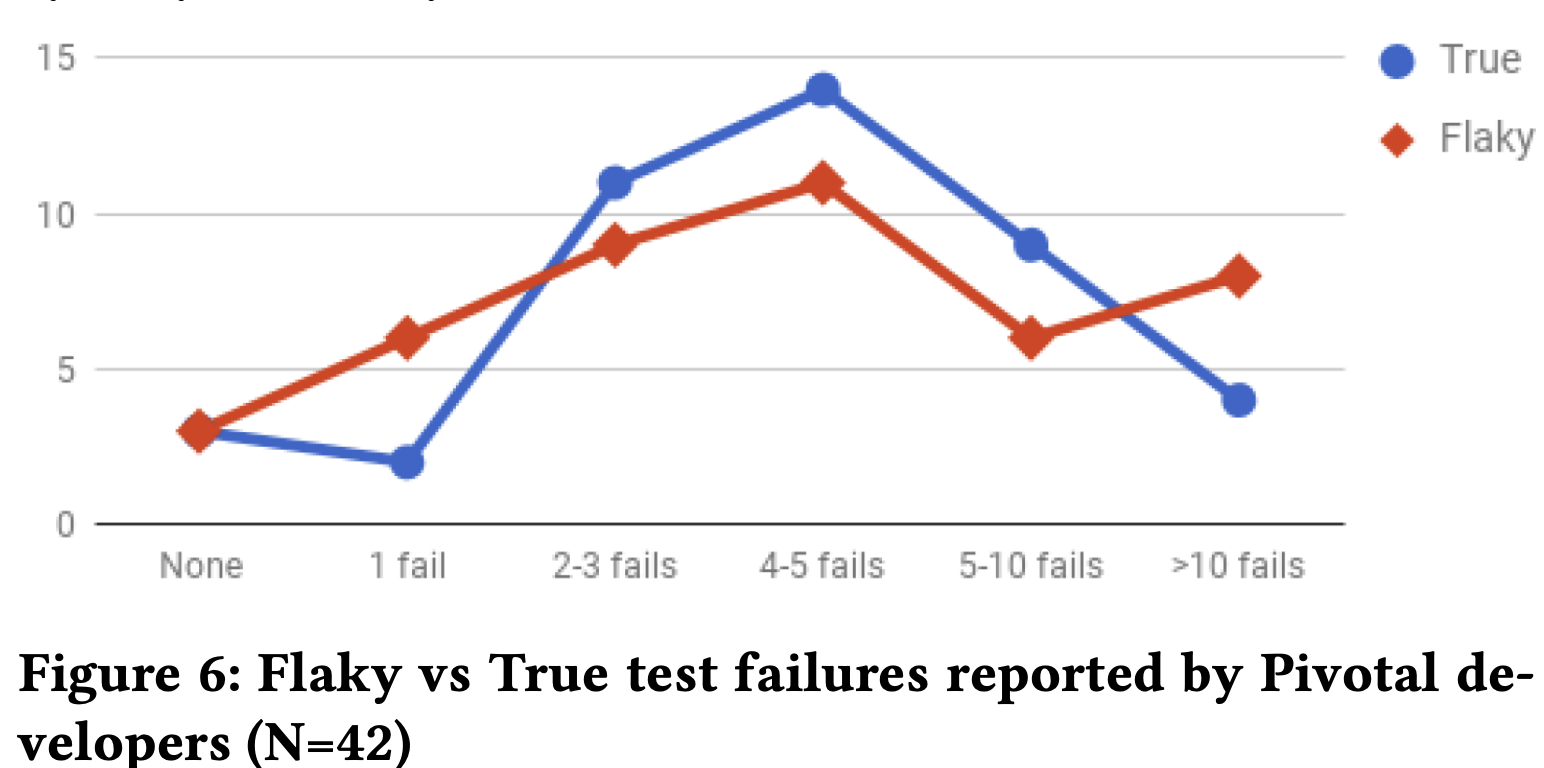
\includegraphics[width=.9\linewidth]{flaky.png}
  \par\columnbreak\par
  ``Pivotal developers experienced similar numbers of flaky and true CI failures per week. However, for the largest category, \ul{>10 fails a week}, there were twice as many flaky failures as true failures.''
  \source{hilton2017trade}
  \end{multicols}}

\end{document}
